\section{Engagement}

Studying engagement on TikTok can reveal how many people are reached and the approval rate of content.

Each post (in this case, only videos) includes several pieces of information that can be used to analyze the content's impact. For example, the API returns data such as the number of views, comments, likes, shares, and more.

Naturally, views have the highest numbers, followed by likes and comments. For these video topics, there is a very low "repost" rate (called shares), which refers to users reposting influencers' video.

In the analysis, some attributes has been normalized thus to obtain a graph well formed.
In detail: views, likes, comments are reported in thousands

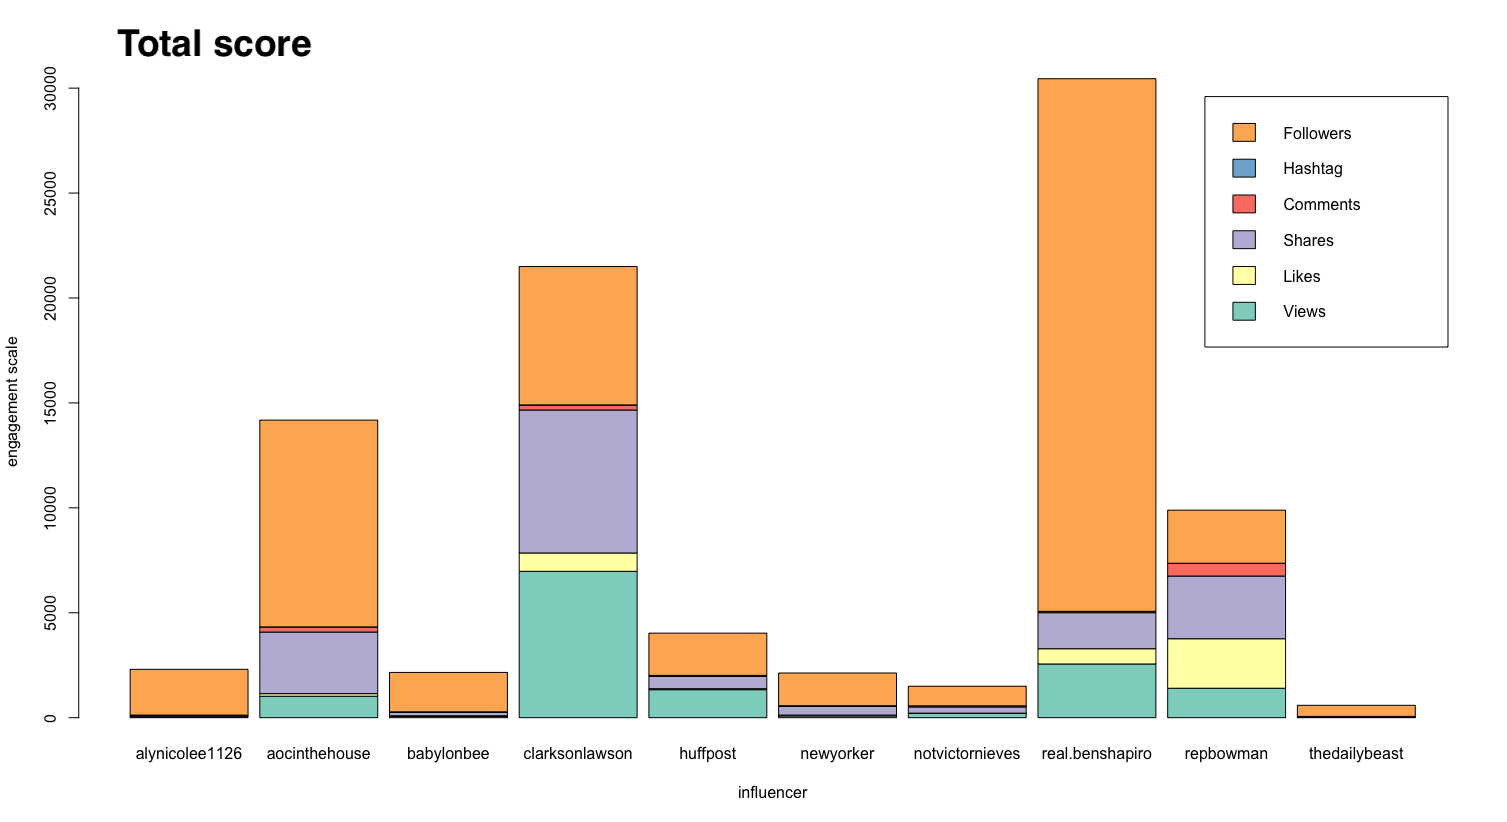
\includegraphics[width = .48\textwidth]{images/Final_Engagement_TotalScore.png}

To compare the two political wings, the data has been divided into two subgroups based on the side of influencers.

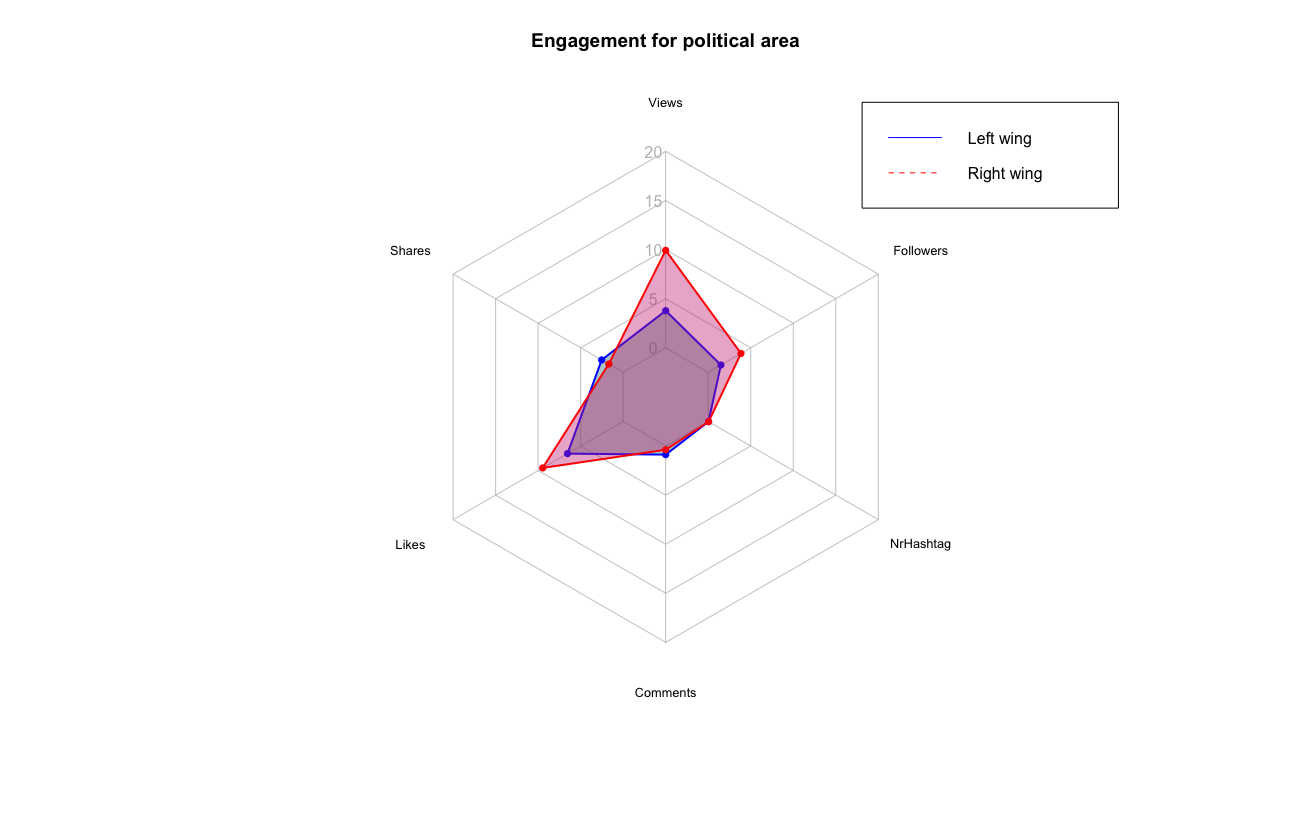
\includegraphics[width = .48\textwidth]{images/Final_Engagement_EngegementPerArea.png}